\chapter{Matrices}\label{app:matrices}

In mathematics, a matrix is a rectangular array of
numbers, symbols, or expressions, arranged in rows and columns. Matrices
are commonly written in box brackets. The horizontal and vertical lines
of entries in a matrix are called rows and columns, respectively. The
size of a matrix is defined by the number of rows and columns that it
contains. A matrix with \(m\) rows and \(n\) columns is called an
\(m\times n\) matrix or \(m\)-by-\(n\) matrix, while \(m\) and \(n\) are
called its dimensions. The dimensions of the following matrix are
\(2\times 3\) (read ``two by three''), because there are two rows and
three columns.

\[\begin{bmatrix}
1 & 2 & 3\\
4 & 5 & 6
\end{bmatrix}\]

The individual items (numbers, symbols or expressions) in a matrix are
called its elements or entries.

In \texttt{python} matrices can be represented as \texttt{numpy.array},
so the example above will become:

\begin{tcolorbox}[breakable, size=fbox, boxrule=1pt, pad at break*=1mm,colback=cellbackground, colframe=cellborder]
\begin{Verbatim}[commandchars=\\\{\}]
\PY{k+kn}{import} \PY{n+nn}{numpy} \PY{k}{as} \PY{n+nn}{np}

\PY{n+nb}{print} \PY{p}{(}\PY{n}{np}\PY{o}{.}\PY{n}{array}\PY{p}{(}\PY{p}{[}\PY{p}{[}\PY{l+m+mi}{1}\PY{p}{,}\PY{l+m+mi}{2}\PY{p}{,}\PY{l+m+mi}{3}\PY{p}{]}\PY{p}{,}\PY{p}{[}\PY{l+m+mi}{4}\PY{p}{,}\PY{l+m+mi}{5}\PY{p}{,}\PY{l+m+mi}{6}\PY{p}{]}\PY{p}{]}\PY{p}{)}\PY{p}{)}

[[1 2 3]
 [4 5 6]]
\end{Verbatim}
\end{tcolorbox}

Essentially a \texttt{numpy.array} is a list of lists each one
representing a matrix row. Arrays can have any dimension so they can be
used to represent also vectors in \texttt{python}. There are two special
types of arrays \texttt{zeros} and \texttt{ones} whose name already
clarify their meaning:

\begin{tcolorbox}[breakable, size=fbox, boxrule=1pt, pad at break*=1mm,colback=cellbackground, colframe=cellborder]
\begin{Verbatim}[commandchars=\\\{\}]
\PY{n}{A} \PY{o}{=} \PY{n}{np}\PY{o}{.}\PY{n}{zeros}\PY{p}{(}\PY{n}{shape}\PY{o}{=}\PY{p}{(}\PY{l+m+mi}{3}\PY{p}{,} \PY{l+m+mi}{3}\PY{p}{)}\PY{p}{)}
\PY{n}{B} \PY{o}{=} \PY{n}{np}\PY{o}{.}\PY{n}{ones}\PY{p}{(}\PY{n}{shape}\PY{o}{=}\PY{p}{(}\PY{l+m+mi}{4}\PY{p}{,} \PY{l+m+mi}{4}\PY{p}{)}\PY{p}{)}

\PY{n+nb}{print} \PY{p}{(}\PY{n}{A}\PY{p}{)}
\PY{n+nb}{print} \PY{p}{(}\PY{n}{B}\PY{p}{)}

[[0. 0. 0.]
 [0. 0. 0.]
 [0. 0. 0.]]

[[1. 1. 1. 1.]
 [1. 1. 1. 1.]
 [1. 1. 1. 1.]
 [1. 1. 1. 1.]]
    \end{Verbatim}
\end{tcolorbox}

\section{Transpose of a Matrix}
The transpose of a matrix $[A]$, denoted by $[A^T]$, may be constructed by writing the rows of $[A]$ as the columns of $[A^T]$
and the columns of $[A]$ as the rows of $[A^T]$.
Formally, the $i$-th row, $j$-th column element of $[A^T]$ is the $j$-th row, $i$-th column element of $[A]$:

\begin{equation}[A^T]_{ij} = [A]_{ji}\end{equation}

If $[A]$ is an $m\times n$ matrix, then $[A^T]$ is an $n\times m$ matrix. 
As an example the transpose of:

\[
\begin{bmatrix}
1 & 5 & 3 \\
2 & -3 & 8
\end{bmatrix}
\quad \mathrm{is} \quad
\begin{bmatrix}
1 & 2 \\
5 & -3 \\
3  & 8
\end{bmatrix}
\]

\section{Operation with Matrices}
\subsection{Adding and Subtracting Matrices}\label{adding-and-subtracting-matrices}

We use matrices to list data or to represent systems. Because the
entries are numbers, we can perform operations on matrices. We add or
subtract matrices by adding or subtracting corresponding entries.

In order to do this, the entries must correspond. Therefore, addition
and subtraction of matrices is only possible when the matrices have the
same dimensions.\\
Adding matrices is very simple. Just add each element in the first
matrix to the corresponding element in the second matrix.

\[
\begin{bmatrix}
1 & 2 & 3 \\
4 & 5 & 6
\end{bmatrix}
+
\begin{bmatrix}
10 & 20 & 30\\
40 & 50 & 60
\end{bmatrix}
=
\begin{bmatrix}
11 & 22 & 33\\
44 & 55 & 66
\end{bmatrix}
\]

As you might guess, subtracting works much the same way except that you
subtract instead of adding.

\[
\begin{bmatrix}
10 & 20 & 30\\
40 & 50 & 60
\end{bmatrix}
-
\begin{bmatrix}
1 & 2 & 3 \\
4 & 5 & 6
\end{bmatrix}
=
\begin{bmatrix}
9 & 18 & 27\\
36 & 45 & 54
\end{bmatrix}
\]

Adding and subtracting \texttt{numpy.array} is as easy as that:

\begin{tcolorbox}[breakable, size=fbox, boxrule=1pt, pad at break*=1mm,colback=cellbackground, colframe=cellborder]
\begin{Verbatim}[commandchars=\\\{\}]
\PY{n}{A} \PY{o}{=} \PY{n}{np}\PY{o}{.}\PY{n}{array}\PY{p}{(}\PY{p}{[}\PY{p}{[}\PY{l+m+mi}{1}\PY{p}{,}\PY{l+m+mi}{2}\PY{p}{,}\PY{l+m+mi}{3}\PY{p}{]}\PY{p}{,}\PY{p}{[}\PY{l+m+mi}{4}\PY{p}{,}\PY{l+m+mi}{5}\PY{p}{,}\PY{l+m+mi}{6}\PY{p}{]}\PY{p}{]}\PY{p}{)}
\PY{n}{B} \PY{o}{=} \PY{n}{np}\PY{o}{.}\PY{n}{array}\PY{p}{(}\PY{p}{[}\PY{p}{[}\PY{l+m+mi}{10}\PY{p}{,}\PY{l+m+mi}{20}\PY{p}{,}\PY{l+m+mi}{30}\PY{p}{]}\PY{p}{,}\PY{p}{[}\PY{l+m+mi}{40}\PY{p}{,}\PY{l+m+mi}{50}\PY{p}{,}\PY{l+m+mi}{60}\PY{p}{]}\PY{p}{]}\PY{p}{)}

\PY{n+nb}{print} \PY{p}{(}\PY{n}{A}\PY{o}{+}\PY{n}{B}\PY{p}{)}
\PY{n+nb}{print} \PY{p}{(}\PY{n}{B}\PY{o}{\PYZhy{}}\PY{n}{A}\PY{p}{)}

[[11 22 33]
 [44 55 66]]
 
[[ 9 18 27]
 [36 45 54]]
    \end{Verbatim}
\end{tcolorbox}

\subsection{Scalar Multiplication}\label{scalar-multiplication}

Multiplying a matrix by a scalar \(c\) means you add the matrix to
itself \(c\) times, or simply multiply each element by that constant.

\[
3 \cdot
\begin{bmatrix}
1 & 2 & 3 \\
4 & 5 & 6
\end{bmatrix}
=
\begin{bmatrix}
3 & 6 & 9 \\
12 & 15 & 18
\end{bmatrix}
\]

Scalar multiplication of \texttt{numpy.array} is:

\begin{tcolorbox}[breakable, size=fbox, boxrule=1pt, pad at break*=1mm,colback=cellbackground, colframe=cellborder]
\begin{Verbatim}[commandchars=\\\{\}]
\PY{n}{c} \PY{o}{=} \PY{l+m+mi}{3}
\PY{n}{A} \PY{o}{=} \PY{n}{np}\PY{o}{.}\PY{n}{array}\PY{p}{(}\PY{p}{[}\PY{p}{[}\PY{l+m+mi}{1}\PY{p}{,}\PY{l+m+mi}{2}\PY{p}{,}\PY{l+m+mi}{3}\PY{p}{]}\PY{p}{,}\PY{p}{[}\PY{l+m+mi}{4}\PY{p}{,}\PY{l+m+mi}{5}\PY{p}{,}\PY{l+m+mi}{6}\PY{p}{]}\PY{p}{]}\PY{p}{)}

\PY{n+nb}{print} \PY{p}{(}\PY{n}{c}\PY{o}{*}\PY{n}{A}\PY{p}{)}

[[ 3  6  9]
 [12 15 18]]
    \end{Verbatim}
\end{tcolorbox}

\subsection{Matrix Multiplication}\label{matrix-multiplication}

Matrix multiplication is multiplying every element of each row of the
first matrix times every element of each column in the second matrix.
When multiplying matrices, the elements of the rows in the first matrix
are multiplied with corresponding columns in the second matrix. Each
entry of the resultant matrix is computed one at a time.

Let's see with an example: \[ 
\begin{bmatrix}
1 & 2 \\
3 & 4
\end{bmatrix}
\cdot
\begin{bmatrix}
5 & 6 \\
7 & 8
\end{bmatrix}
= ?
\]

First ask: do the number of columns in the first matrix equal the number
of rows in the second ? If so the product exists. Then start with
producing the product for the first row, first column element. Take the
first row of the first matrix and multiply by the first column of the
second like this:

\[ 
\begin{bmatrix}
1 & 2 \\
3 & 4
\end{bmatrix}
\cdot
\begin{bmatrix}
5 & 6 \\
7 & 8
\end{bmatrix}
=
\begin{bmatrix}
(1\cdot 5) + (2\cdot 7) & X \\
X & X
\end{bmatrix}
\]

Continue the pattern with the first row of the first matrix with the
second column of the second matrix:

\[ 
\begin{bmatrix}
1 & 2 \\
3 & 4
\end{bmatrix}
\cdot
\begin{bmatrix}
5 & 6 \\
7 & 8
\end{bmatrix}
=
\begin{bmatrix}
(1\cdot 5) + (2\cdot 7) & (1\cdot 6) + (2\cdot 8)  \\
X & X
\end{bmatrix}
\]

The do the same with the second row of the first matrix and you are
done:

\[ 
\begin{bmatrix}
1 & 2 \\
3 & 4
\end{bmatrix}
\cdot
\begin{bmatrix}
5 & 6 \\
7 & 8
\end{bmatrix}
=
\begin{bmatrix}
(1\cdot 5) + (2\cdot 7) & (1\cdot 6) + (2\cdot 8)  \\
(3\cdot 5) + (4\cdot 7) & (3\cdot 6) + (4\cdot 8) 
\end{bmatrix}
=
\begin{bmatrix}
19 & 22 \\
43 & 50 
\end{bmatrix}
\]

In \texttt{numpy} array multiplication can be done like this:

\begin{tcolorbox}[breakable, size=fbox, boxrule=1pt, pad at break*=1mm,colback=cellbackground, colframe=cellborder]
\begin{Verbatim}[commandchars=\\\{\}]
\PY{n}{A} \PY{o}{=} \PY{n}{np}\PY{o}{.}\PY{n}{array}\PY{p}{(}\PY{p}{[}\PY{p}{[}\PY{l+m+mi}{1}\PY{p}{,}\PY{l+m+mi}{2}\PY{p}{]}\PY{p}{,}\PY{p}{[}\PY{l+m+mi}{3}\PY{p}{,}\PY{l+m+mi}{4}\PY{p}{]}\PY{p}{]}\PY{p}{)}
\PY{n}{B} \PY{o}{=} \PY{n}{np}\PY{o}{.}\PY{n}{array}\PY{p}{(}\PY{p}{[}\PY{p}{[}\PY{l+m+mi}{5}\PY{p}{,}\PY{l+m+mi}{6}\PY{p}{]}\PY{p}{,}\PY{p}{[}\PY{l+m+mi}{7}\PY{p}{,}\PY{l+m+mi}{8}\PY{p}{]}\PY{p}{]}\PY{p}{)}

\PY{n+nb}{print} \PY{p}{(}\PY{n}{np}\PY{o}{.}\PY{n}{dot}\PY{p}{(}\PY{n}{A}\PY{p}{,} \PY{n}{B}\PY{p}{)}\PY{p}{)}

[[19 22]
 [43 50]]
    \end{Verbatim}
\end{tcolorbox}

\section{The identity matrix}\label{the-identity-matrix}

\([I]\) is defined so that \([A][I]=[A]\), i.e.~it is the matrix version
of multiplying a number by one. What matrix has this property? A first
guess might be a matrix full of 1s, but that does not work:

\[
\begin{bmatrix}
1 & 2 \\
3 & 4
\end{bmatrix}
\begin{bmatrix}
1 & 1 \\
1 & 1
\end{bmatrix}
=
\begin{bmatrix}
3 & 3 \\
7 & 7
\end{bmatrix}
\]

So our initial guess was wrong ! The matrix that does work is a diagonal
stretch of 1s, with all other elements being 0:

\[
\begin{bmatrix}
1 & 2 \\
3 & 4
\end{bmatrix}
\begin{bmatrix}
1 & 0 \\
0 & 1
\end{bmatrix}
=
\begin{bmatrix}
1 & 2 \\
3 & 4
\end{bmatrix}
\]

So \([I] = 
\begin{bmatrix}
1 & 0 \\
0 & 1
\end{bmatrix}
\) is the identity matrix for \(2\times 2\) matrices.

The \texttt{numpy} equivalent of the identity matrix is given by
\texttt{numpy.identity(n)} with n the dimension of the matrix. So for
example:

\begin{tcolorbox}[breakable, size=fbox, boxrule=1pt, pad at break*=1mm,colback=cellbackground, colframe=cellborder]
\begin{Verbatim}[commandchars=\\\{\}]
\PY{n}{A} \PY{o}{=} \PY{n}{np}\PY{o}{.}\PY{n}{array}\PY{p}{(}\PY{p}{[}\PY{p}{[}\PY{l+m+mi}{1}\PY{p}{,}\PY{l+m+mi}{2}\PY{p}{]}\PY{p}{,}\PY{p}{[}\PY{l+m+mi}{3}\PY{p}{,}\PY{l+m+mi}{4}\PY{p}{]}\PY{p}{]}\PY{p}{)}
\PY{n}{I} \PY{o}{=} \PY{n}{np}\PY{o}{.}\PY{n}{identity}\PY{p}{(}\PY{l+m+mi}{2}\PY{p}{)}

\PY{n+nb}{print} \PY{p}{(}\PY{n}{A}\PY{p}{)}
\PY{n+nb}{print} \PY{p}{(}\PY{p}{)}
\PY{n+nb}{print} \PY{p}{(}\PY{n}{np}\PY{o}{.}\PY{n}{dot}\PY{p}{(}\PY{n}{A}\PY{p}{,} \PY{n}{I}\PY{p}{)}\PY{p}{)}

[[1 2]
 [3 4]]

[[1. 2.]
 [3. 4.]]
    \end{Verbatim}
\end{tcolorbox}

    
\section{Matrix Decomposition}
\label{eigendecomposition}

Decomposing a matrix means that we want to find a product of matrices that is equal to the initial matrix. 
In this Section the case of \emph{eigen-decomposition} is described, 
where we decompose the initial matrix into the product of its \emph{eigenvectors} and \emph{eigenvalues}.
%Before all, let's see the link between matrices and linear
%transformation. Then, you'll learn what are eigenvectors and
%eigenvalues.

\subsection{Eigenvectors and eigenvalues}
\label{eigenvectors-and-eigenvalues}
%\subsection{Matrices as linear transformations}
%\label{matrices-as-linear-transformations}

You can think of matrices as linear transformations. Some matrices will
rotate your space, others will re-scale it. When we apply a matrix to a
vector (apply here means calculate the
dot product of the matrix with the vector), we end up with a transformed version of the vector.

Let's apply the matrix \([A]\) to a vector $\mathbf{v}$

\begin{tcolorbox}[breakable, size=fbox, boxrule=1pt, pad at break*=1mm,colback=cellbackground, colframe=cellborder]
\begin{Verbatim}[commandchars=\\\{\}]
\PY{k+kn}{import} \PY{n+nn}{numpy} \PY{k}{as} \PY{n+nn}{np}
\PY{k+kn}{from} \PY{n+nn}{finmarkets} \PY{k}{import} \PY{n}{plotVectors}
\PY{k+kn}{from} \PY{n+nn}{matplotlib} \PY{k}{import} \PY{n}{pyplot} \PY{k}{as} \PY{n}{plt}
	
\PY{n}{A} \PY{o}{=} \PY{n}{np}\PY{o}{.}\PY{n}{array}\PY{p}{(}\PY{p}{[}\PY{p}{[}\PY{o}{\PYZhy{}}\PY{l+m+mi}{1}\PY{p}{,} \PY{l+m+mi}{3}\PY{p}{]}\PY{p}{,} \PY{p}{[}\PY{l+m+mi}{2}\PY{p}{,} \PY{o}{\PYZhy{}}\PY{l+m+mi}{2}\PY{p}{]}\PY{p}{]}\PY{p}{)}
\PY{n}{v} \PY{o}{=} \PY{n}{np}\PY{o}{.}\PY{n}{array}\PY{p}{(}\PY{p}{[}\PY{p}{[}\PY{l+m+mi}{2}\PY{p}{]}\PY{p}{,} \PY{p}{[}\PY{l+m+mi}{1}\PY{p}{]}\PY{p}{]}\PY{p}{)}	
\PY{n}{Av} \PY{o}{=} \PY{n}{A}\PY{o}{.}\PY{n}{dot}\PY{p}{(}\PY{n}{v}\PY{p}{)}
	
\PY{n}{plotVectors}\PY{p}{(}\PY{p}{[}\PY{n}{v}\PY{o}{.}\PY{n}{flatten}\PY{p}{(}\PY{p}{)}\PY{p}{,} \PY{n}{Av}\PY{o}{.}\PY{n}{flatten}\PY{p}{(}\PY{p}{)}\PY{p}{]}\PY{p}{,} \PY{n}{cols}\PY{o}{=}\PY{p}{[}\PY{l+s+s1}{\PYZsq{}}\PY{l+s+s1}{\PYZsh{}1190FF}\PY{l+s+s1}{\PYZsq{}}\PY{p}{,} \PY{l+s+s1}{\PYZsq{}}\PY{l+s+s1}{\PYZsh{}FF9A13}\PY{l+s+s1}{\PYZsq{}}\PY{p}{]}\PY{p}{)}
\PY{n}{plt}\PY{o}{.}\PY{n}{ylim}\PY{p}{(}\PY{o}{\PYZhy{}}\PY{l+m+mi}{1}\PY{p}{,} \PY{l+m+mi}{4}\PY{p}{)}
\PY{n}{plt}\PY{o}{.}\PY{n}{xlim}\PY{p}{(}\PY{o}{\PYZhy{}}\PY{l+m+mi}{1}\PY{p}{,} \PY{l+m+mi}{4}\PY{p}{)}

(-1.0, 4.0)
\end{Verbatim}
\end{tcolorbox}

Figure~\ref{fig:matrix_as_transform} shows the effect of the application of the matrix to the vector, the new vector (orange) has a different direction than the original one (light blue).

\begin{figure}[htb]
	\centering
	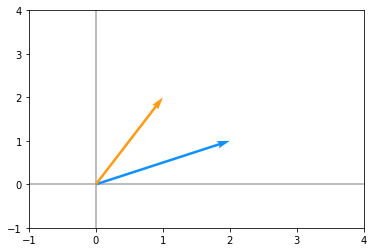
\includegraphics[width=0.7\linewidth]{figures/matrix_transformation}
	\caption{Application of a matrix to a vector, the new vector (orange) is different than the original one (blue).}
	\label{fig:matrix_as_transform}
\end{figure}


%We have seen an example of a vector transformed by a matrix. Now
%imagine that the transformation of the initial \%vector gives us a new
%vector that has the exact same direction. The scale can be different but
%the direction is the \%same. Applying the matrix doesn't change the
%direction of the vector. This special vector is called an eigenvector of
%\%the matrix.

Now imagine that the transformation of the initial vector by the matrix
gives a new vector with the exact same direction. This vector is called
an \emph{eigenvector} of \([A]\).

This means that \textbf{v} is a eigenvector of \([A]\) if \textbf{v} and \([A]\mathbf{v}\)
(the transformed vector) are in the same direction. The output vector is
just a scaled version of the input vector with a the scaling factor
\(\lambda\) which is called an \emph{eigenvalue} of \([A]\).
Mathematically, we have the following equation:

\begin{equation}
[A]\mathbf{v}=\lambda \mathbf{v}
\end{equation}

\subsection{Finding Eigenvalues and Eigenvectors in \texttt{python}}
\label{find-eigenvalues-and-eigenvectors-in-python}

\(\tt{numpy}\) provides a function returning eigenvectors and
eigenvalues: 

\begin{tcolorbox}[breakable, size=fbox, boxrule=1pt, pad at break*=1mm,colback=cellbackground, colframe=cellborder]
\begin{Verbatim}[commandchars=\\\{\}]
\PY{n}{A} \PY{o}{=} \PY{n}{np}\PY{o}{.}\PY{n}{array}\PY{p}{(}\PY{p}{[}\PY{p}{[}\PY{l+m+mi}{5}\PY{p}{,} \PY{l+m+mi}{1}\PY{p}{]}\PY{p}{,} \PY{p}{[}\PY{l+m+mi}{3}\PY{p}{,} \PY{l+m+mi}{3}\PY{p}{]}\PY{p}{]}\PY{p}{)}
\PY{n}{np}\PY{o}{.}\PY{n}{linalg}\PY{o}{.}\PY{n}{eig}\PY{p}{(}\PY{n}{A}\PY{p}{)}
	
(array([6., 2.]),
array([[ 0.70710678, -0.31622777],
       [ 0.70710678,  0.9486833 ]]))
\end{Verbatim}
\end{tcolorbox}
The eigenvectors correspond to the columns of the second array. This
means that the eigenvector corresponding to \(\lambda=6\) is:

\[\begin{bmatrix}
0.70710678 \\
0.70710678\end{bmatrix}\]
while the eigenvector corresponding to \(\lambda=2\) is:

\[\begin{bmatrix}
−0.31622777 \\
0.9486833\end{bmatrix}\]

It is important to note that there exists an infinite number of 
eigenvectors corresponding to a given eigenvalue, they are equivalent
because they have the same direction but are just scaled differently.
For example the first eigenvector found above is a scaled version of
\(\begin{bmatrix}1\\ 1\end{bmatrix}\).

\begin{tcolorbox}[breakable, size=fbox, boxrule=1pt, pad at break*=1mm,colback=cellbackground, colframe=cellborder]
\begin{Verbatim}[commandchars=\\\{\}]
\PY{n}{v} \PY{o}{=} \PY{n}{np}\PY{o}{.}\PY{n}{array}\PY{p}{(}\PY{p}{[}\PY{p}{[}\PY{l+m+mi}{1}\PY{p}{]}\PY{p}{,} \PY{p}{[}\PY{o}{\PYZhy{}}\PY{l+m+mi}{3}\PY{p}{]}\PY{p}{]}\PY{p}{)}
\PY{n}{Av} \PY{o}{=} \PY{n}{A}\PY{o}{.}\PY{n}{dot}\PY{p}{(}\PY{n}{v}\PY{p}{)}
\PY{n}{v\PYZus{}np} \PY{o}{=} \PY{p}{[}\PY{o}{\PYZhy{}}\PY{l+m+mf}{0.31622777}\PY{p}{,} \PY{l+m+mf}{0.9486833}\PY{p}{]}	
	
(-1.0, 3.0)
\end{Verbatim}
\end{tcolorbox}
Figure~\ref{fig:eigenvectors} shows three equivalent eigenvectors found
with the code above. We can see that the vector found with \(\tt{numpy}\) (in dark blue) is a scaled version of \(\begin{bmatrix}1\\ -3\end{bmatrix}\).

\begin{figure}[htb]
	\centering
	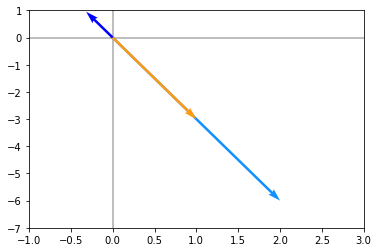
\includegraphics[width=0.7\linewidth]{figures/eigenvectors}
	\caption{Graphical representation of three equivalent eigenvectors.}
	\label{fig:eigenvectors}
\end{figure}

%Let's \([A]\) be the following matrix:
%
%\[A=\begin{bmatrix}
%5 &1 \\
%3 &3
%\end{bmatrix}\]
%
%We know that one eigenvector of A is:
%
%\[v=\begin{bmatrix}
%1 \\
%1\end{bmatrix}\] We can check that \([A]v=\lambda v\)
%
%\[\begin{bmatrix}
%5 & 1 \\
%3& 3\end{bmatrix}
%\begin{bmatrix}
%1 \\
%1\end{bmatrix}
%=\begin{bmatrix}
%6 \\
%6\end{bmatrix}\]
%
%We can represent \(v\) and \([A]v\) to check if their directions are the
%same:
%
%\begin{tcolorbox}[breakable, size=fbox, boxrule=1pt, pad at break*=1mm,colback=cellbackground, colframe=cellborder]
%	\begin{Verbatim}[commandchars=\\\{\}]
%	\PY{n}{A} \PY{o}{=} \PY{n}{np}\PY{o}{.}\PY{n}{array}\PY{p}{(}\PY{p}{[}\PY{p}{[}\PY{l+m+mi}{5}\PY{p}{,} \PY{l+m+mi}{1}\PY{p}{]}\PY{p}{,} \PY{p}{[}\PY{l+m+mi}{3}\PY{p}{,} \PY{l+m+mi}{3}\PY{p}{]}\PY{p}{]}\PY{p}{)}
%	\PY{n}{v} \PY{o}{=} \PY{n}{np}\PY{o}{.}\PY{n}{array}\PY{p}{(}\PY{p}{[}\PY{p}{[}\PY{l+m+mi}{1}\PY{p}{]}\PY{p}{,} \PY{p}{[}\PY{l+m+mi}{1}\PY{p}{]}\PY{p}{]}\PY{p}{)}
%	
%	\PY{n}{Av} \PY{o}{=} \PY{n}{A}\PY{o}{.}\PY{n}{dot}\PY{p}{(}\PY{n}{v}\PY{p}{)}
%	
%	\PY{n}{orange} \PY{o}{=} \PY{l+s+s1}{\PYZsq{}}\PY{l+s+s1}{\PYZsh{}FF9A13}\PY{l+s+s1}{\PYZsq{}}
%	\PY{n}{blue} \PY{o}{=} \PY{l+s+s1}{\PYZsq{}}\PY{l+s+s1}{\PYZsh{}1190FF}\PY{l+s+s1}{\PYZsq{}}
%	
%	\PY{n}{plotVectors}\PY{p}{(}\PY{p}{[}\PY{n}{Av}\PY{o}{.}\PY{n}{flatten}\PY{p}{(}\PY{p}{)}\PY{p}{,} \PY{n}{v}\PY{o}{.}\PY{n}{flatten}\PY{p}{(}\PY{p}{)}\PY{p}{]}\PY{p}{,} \PY{n}{cols}\PY{o}{=}\PY{p}{[}\PY{n}{blue}\PY{p}{,} \PY{n}{orange}\PY{p}{]}\PY{p}{)}
%	\PY{n}{plt}\PY{o}{.}\PY{n}{ylim}\PY{p}{(}\PY{o}{\PYZhy{}}\PY{l+m+mi}{1}\PY{p}{,} \PY{l+m+mi}{7}\PY{p}{)}
%	\PY{n}{plt}\PY{o}{.}\PY{n}{xlim}\PY{p}{(}\PY{o}{\PYZhy{}}\PY{l+m+mi}{1}\PY{p}{,} \PY{l+m+mi}{7}\PY{p}{)}
%
%(-1.0, 7.0)
%\end{Verbatim}
%\end{tcolorbox}
%
%\begin{center}
%	\adjustimage{max size={0.9\linewidth}{0.9\paperheight}}{eigenvectors_files/eigenvectors_3_1.png}
%\end{center}
%
%We can see that their directions are the same!
%
%This example shows that the eigenvectors \(v\) are vectors that change
%only in scale when we apply the matrix \([A]\) to them.

\section{The Inverse of a Matrix}\label{the-inverse-of-a-matrix}

The inverse of matrix \([A]\) is \([A^{-1}]\), and is defined by the
property:

\begin{equation} [A][A^{-1}]=[I] \end{equation}

Hence the matrix \([B]\) is the inverse of the matrix \([A]\) if when
multiplied together, \([A][B]\) gives the identity matrix. 

Using the definition let's try to find the inverse of:

\[
\begin{bmatrix}
3 & 4\\
5 & 6
\end{bmatrix}
\]

First, let the following be true:

\[
\begin{bmatrix}
3 & 4\\
5 & 6
\end{bmatrix}
\begin{bmatrix}
a & b\\
c & d
\end{bmatrix}
=
\begin{bmatrix}
1 & 0\\
0 & 1
\end{bmatrix}
\]
When multiplying this mystery matrix by our original matrix, the result is

\[
\begin{bmatrix}
3a+4c & 3b+4d\\
5a+6c & 5b+6d
\end{bmatrix}
=
\begin{bmatrix}
1 & 0\\
0 & 1
\end{bmatrix}
\]
For two matrices to be equal, every element in the left must equal its
corresponding element on the right. So, for these two matrices to equal
each other:

\[
\begin{cases}
3a+4c=1\\
3b+4d=0\\
5a+6c=0\\
5b+6d=1
\end{cases}
\]
Solving this simple system we get the following result:

\[
\begin{cases}
a=−3\\
b=2\\
c=2.5\\
d=−1.5
\end{cases}
\]
Having solved for the four variables, the result is the inverse

\[
\begin{bmatrix}
−3 & 2\\
2.5 & −1.5
\end{bmatrix}
\]
The quick check to be sure the result is correct is done in \texttt{python}.
The \texttt{linalg.inv()} function can be used to find the inverse of a
matrix:

\begin{tcolorbox}[breakable, size=fbox, boxrule=1pt, pad at break*=1mm,colback=cellbackground, colframe=cellborder]
	\begin{Verbatim}[commandchars=\\\{\}]
	\PY{k+kn}{from} \PY{n+nn}{numpy}\PY{n+nn}{.}\PY{n+nn}{linalg} \PY{k}{import} \PY{n}{inv}
	
	\PY{n}{A} \PY{o}{=} \PY{n}{np}\PY{o}{.}\PY{n}{array}\PY{p}{(}\PY{p}{[}\PY{p}{[}\PY{l+m+mi}{3}\PY{p}{,}\PY{l+m+mi}{4}\PY{p}{]}\PY{p}{,}\PY{p}{[}\PY{l+m+mi}{5}\PY{p}{,}\PY{l+m+mi}{6}\PY{p}{]}\PY{p}{]}\PY{p}{)}
	\PY{n+nb}{print} \PY{p}{(}\PY{n}{inv}\PY{p}{(}\PY{n}{A}\PY{p}{)}\PY{p}{)}
	
	[[-3.   2. ]
	[ 2.5 -1.5]]
	\end{Verbatim}
\end{tcolorbox}

\subsection{The Moore-Penrose Pseudo-inverse}
\label{the-moore-penrose-pseudoinverse}

%The Moore-Penrose pseudo-inverse is a direct application of the SVD. But
%before all, we have to remind that systems of equations can be expressed
%under the matrix form.
The Moore-Penrose pseudo-inverse is \([A^+]\) such as:

\[[A][A^+]≈[I]\]

Think of it as a generalization of the inverse. It is defined for all
matrices, but has fewer guaranteed properties as a result. For example,
it will be a matrix such that \([𝐴][𝐴^+][𝐴]=[𝐴]\), but not necessarily
the stronger usual inverse property is true \([𝐴^{−1}][𝐴]=[𝐴][𝐴^{−1}]=[𝐼]\) (the second one implies the first). In the special case where a matrix has an inverse, it will be the same as the pseudo-inverse.

%So pinv() gives you the inverse where it exists, and still gives
%something inverse-like everywhere else.

%The pseudo-inverse is the ``closest'' answer to \([𝐴]\mathbf{x}=[𝐼]\), in the sense that the norm \(||[𝐴][𝑋]−[𝐼]||_2\) is smallest. It's 0 when the
%inverse exists of course.

Let's create a non square matrix $[A]$, calculate its singular value decomposition and its pseudo-inverse.

\[A=\begin{bmatrix}
7&2\\
3&4\\
5&3\end{bmatrix}\]

\begin{tcolorbox}[breakable, size=fbox, boxrule=1pt, pad at break*=1mm,colback=cellbackground, colframe=cellborder]
\begin{Verbatim}[commandchars=\\\{\}]
\PY{n}{A} \PY{o}{=} \PY{n}{np}\PY{o}{.}\PY{n}{array}\PY{p}{(}\PY{p}{[}\PY{p}{[}\PY{l+m+mi}{7}\PY{p}{,} \PY{l+m+mi}{2}\PY{p}{]}\PY{p}{,} \PY{p}{[}\PY{l+m+mi}{3}\PY{p}{,} \PY{l+m+mi}{4}\PY{p}{]}\PY{p}{,} \PY{p}{[}\PY{l+m+mi}{5}\PY{p}{,} \PY{l+m+mi}{3}\PY{p}{]}\PY{p}{]}\PY{p}{)}
\PY{n}{A\PYZus{}plus} \PY{o}{=} \PY{n}{np}\PY{o}{.}\PY{n}{linalg}\PY{o}{.}\PY{n}{pinv}\PY{p}{(}\PY{n}{A}\PY{p}{)}
\PY{n+nb}{print} \PY{p}{(}\PY{n}{A\PYZus{}plus}\PY{p}{)}
	
[[ 0.16666667 -0.10606061  0.03030303]
 [-0.16666667  0.28787879  0.06060606]]
	\end{Verbatim}
\end{tcolorbox}
We can now check that it is really the near inverse of $[A]$.
Since we know that

\[[A^{−1}][A]=[I]\]

\begin{tcolorbox}[breakable, size=fbox, boxrule=1pt, pad at break*=1mm,colback=cellbackground, colframe=cellborder]
\begin{Verbatim}[commandchars=\\\{\}]
\PY{n}{A\PYZus{}plus}\PY{o}{.}\PY{n}{dot}\PY{p}{(}\PY{n}{A}\PY{p}{)}
	
array([[1.00000000e+00, 2.35922393e-16],
       [3.33066907e-16, 1.00000000e+00]])
\end{Verbatim}
\end{tcolorbox}
This is almost the identity matrix!
Another difference with respect to the real inverse is that \([A^+][A]≈[I]\) but \([A][A^+]\neq [I]\).

\subsection{Eigen-decomposition}
\label{concatenating-eigenvalues-and-eigenvectors}

Now that we have an idea of what eigenvectors and eigenvalues are, we
can see how it can be used to decompose a matrix. 
Then the \emph{eigen-decomposition} is given by

\begin{equation}
[A]=[V]\cdot \textrm{diag}(\boldsymbol{\lambda})\cdot [V^{−1}]
\end{equation}
where the matrix $[V]$ is made by concatenating all eigenvectors
of $[A]$ in each column (like in the second array returned by
\(\tt{np.linalg.eig(A))}\), \(\textrm{diag}(\boldsymbol{\lambda})\) 
is a diagonal matrix containing all the eigenvalues.
Continuing with our example above we have

\[V=\begin{bmatrix}
1 & 1 \\
1 &−3\end{bmatrix}\qquad 
\textrm{diag}(\boldsymbol{\lambda})=\begin{bmatrix}
6&0\\
0&2\end{bmatrix}\] 
and the inverse matrix of \([V]\) can be calculated with
\(\tt{numpy}\)

\begin{tcolorbox}[breakable, size=fbox, boxrule=1pt, pad at break*=1mm,colback=cellbackground, colframe=cellborder]
\begin{Verbatim}[commandchars=\\\{\}]
\PY{n}{V} \PY{o}{=} \PY{n}{np}\PY{o}{.}\PY{n}{array}\PY{p}{(}\PY{p}{[}\PY{p}{[}\PY{l+m+mi}{1}\PY{p}{,} \PY{l+m+mi}{1}\PY{p}{]}\PY{p}{,} \PY{p}{[}\PY{l+m+mi}{1}\PY{p}{,} \PY{o}{\PYZhy{}}\PY{l+m+mi}{3}\PY{p}{]}\PY{p}{]}\PY{p}{)}
\PY{n}{V\PYZus{}inv} \PY{o}{=} \PY{n}{np}\PY{o}{.}\PY{n}{linalg}\PY{o}{.}\PY{n}{inv}\PY{p}{(}\PY{n}{V}\PY{p}{)}
\PY{n}{V\PYZus{}inv}

array([[ 0.75,  0.25],
       [ 0.25, -0.25]])
\end{Verbatim}
\end{tcolorbox}

So let's plug it into our equation:

\[ [V]\cdot\textrm{diag}(\boldsymbol{\lambda})\cdot [V^{−1}]=
\begin{bmatrix}
1 & 1 \\
1 &−3\end{bmatrix}
\begin{bmatrix}
6&0\\
0&2\end{bmatrix}
\begin{bmatrix}
0.75 & 0.25\\
0.25&-0.25 \end{bmatrix}
=\begin{bmatrix}
5 & 1\\
3& 3\end{bmatrix}
\]

Let's check our result with \texttt{python}

\begin{tcolorbox}[breakable, size=fbox, boxrule=1pt, pad at break*=1mm,colback=cellbackground, colframe=cellborder]
\begin{Verbatim}[commandchars=\\\{\}]
\PY{n}{lambdas} \PY{o}{=} \PY{n}{np}\PY{o}{.}\PY{n}{diag}\PY{p}{(}\PY{p}{[}\PY{l+m+mi}{6}\PY{p}{,} \PY{l+m+mi}{2}\PY{p}{]}\PY{p}{)}
\PY{n}{V}\PY{o}{.}\PY{n}{dot}\PY{p}{(}\PY{n}{lambdas}\PY{p}{)}\PY{o}{.}\PY{n}{dot}\PY{p}{(}\PY{n}{V\PYZus{}inv}\PY{p}{)}

array([[5., 1.],
       [3., 3.]])
\end{Verbatim}
\end{tcolorbox}

\subsubsection{Real symmetric matrix}
\label{real-symmetric-matrix}

In the case of real symmetric matrices (\([A]=[A^T]\)) the
eigen-decomposition can be expressed as

\begin{equation}
[A]=[Q][\Lambda][Q^T]
\end{equation} 
where \([Q]\) is the matrix with eigenvectors
as columns and \(\Lambda\) is \(\textrm{diag}(\boldsymbol{\lambda})\).

For that reason, it can useful to use symmetric matrices! Let's do it
now with \(\tt{linalg}\) from \(\tt{numpy}\)

\begin{tcolorbox}[breakable, size=fbox, boxrule=1pt, pad at break*=1mm,colback=cellbackground, colframe=cellborder]
\begin{Verbatim}[commandchars=\\\{\}]
\PY{n}{A} \PY{o}{=} \PY{n}{np}\PY{o}{.}\PY{n}{array}\PY{p}{(}\PY{p}{[}\PY{p}{[}\PY{l+m+mi}{6}\PY{p}{,} \PY{l+m+mi}{2}\PY{p}{]}\PY{p}{,} \PY{p}{[}\PY{l+m+mi}{2}\PY{p}{,} \PY{l+m+mi}{3}\PY{p}{]}\PY{p}{]}\PY{p}{)}
\PY{n}{eigVals}\PY{p}{,} \PY{n}{eigVecs} \PY{o}{=} \PY{n}{np}\PY{o}{.}\PY{n}{linalg}\PY{o}{.}\PY{n}{eig}\PY{p}{(}\PY{n}{A}\PY{p}{)}
\PY{n}{eigVals} \PY{o}{=} \PY{n}{np}\PY{o}{.}\PY{n}{diag}\PY{p}{(}\PY{n}{eigVals}\PY{p}{)}
\PY{n}{eigVecs}\PY{o}{.}\PY{n}{dot}\PY{p}{(}\PY{n}{eigVals}\PY{p}{)}\PY{o}{.}\PY{n}{dot}\PY{p}{(}\PY{n}{eigVecs}\PY{o}{.}\PY{n}{T}\PY{p}{)}

array([[6., 2.],
       [2., 3.]])
\end{Verbatim}
\end{tcolorbox}

%\subsubsection{Quadratic form to matrix form}
%\label{quadratic-form-to-matrix-form}
%
%Let's have the following quadratic equation:
%
%\[f(x)=ax^2_1+(b+c)x_1x_2+dx^2_2\] These quadratic forms can be
%generated by matrices:
%
%\[f(x)=
%\begin{bmatrix}
%x_1 & x_2
%\end{bmatrix}
%\begin{bmatrix}
%a&b\\
%c&d
%\end{bmatrix}
%\begin{bmatrix}
%x_1\\
%x_2\end{bmatrix}
%=x^T[A]x\]
%
%\subsection{With the Principal Axes Theorem}
%\label{with-the-principal-axes-theorem}
%
%Actually there is a simpler way to do the change of variable. We can
%stay in the matrix form. Recall that we start with the form:
%
%\[f(x)=x^T[A]x\] The linear substitution can be wrote in these terms. We
%want replace the variables \(x\) by \(y\) that relates by:
%
%\[x=[P]y\] We want to find \([P]\) such as our new equation doesn't
%contain the cross terms. The first step is to replace that in the first
%equation:
%
%\[x^T[A]x=([P]y)^T[A]([P]y)=y^T([P]^T[A][P])y\] Can you see the how to
%transform the left hand side (\(x\)) into the right hand side (\(y\))?
%The substitution is done by replacing \([A]\) with \([P]^T[A][P]\). We
%also know that \([A]\) is symmetric and thus that there is a diagonal
%matrix \([D]\) containing the eigenvectors of \([A]\) and such as
%\([D]=[P]^T[A][P]\). We thus end up with:
%
%\[x^T[A]x=y^T[D]y\] All of this implies that we can use \([D]\) to
%simplify our quadratic equation and remove the cross terms. If you
%remember from example 2 we know that the eigenvalues of \([A]\) are:
%
%\[[D]=\begin{bmatrix}
%7 &0\\
%0 &2\end{bmatrix}\]
%
%\[x^T[A]x=y^T[D]y=y^T
%\begin{bmatrix}
%7 &0\\
%0 &2\end{bmatrix}y=
%\begin{bmatrix}y_1 & y_2\end{bmatrix}
%\begin{bmatrix}
%7 &0\\
%0 &2\end{bmatrix}
%\begin{bmatrix}y_1\\y_2\end{bmatrix}
%=\begin{bmatrix}7y_1+0y_2 & 0y_1+2y_2\end{bmatrix}
%\begin{bmatrix}y_1\\y_2\end{bmatrix}=7y^2_1+2y^2_2
%\]
%
%This form (without cross-term) is called the principal axes form.
%
%\subsection{Quadratic form optimization}
%\label{quadratic-form-optimization}
%
%Depending to the context, optimizing a function means finding its
%maximum or its minimum. It is for instance widely used to minimize the
%error of cost functions in machine learning.
%
%Here we will see how eigendecomposition can be used to optimize
%quadratic functions and why this can be done easily without cross terms.
%The difficulty is that we want a constrained optimization, that is to
%find the minimum or the maximum of the function for \(f(x)\) being a
%unit vector.
%
%\paragraph{Example 8.}\label{example-8.}
%
%We want to optimize:
%
%\(f(x)=x^T[A]x\) subject to \(||x||_2=1\).In our last example we ended
%up with:
%
%\(f(x)=7y^2_1+2y^2_2\) And the constraint of \(x\) being a unit vector
%imply:
%
%\[||x||_2=1 \implies x^2_1+x^2_2=1\] We can also show that \(y\) has to
%be a unit vector if it is the case for \(x\). Recall first that
%\(x=[P]y\):
%
%%\[||x||_2=$x^Tx=([P]y)^T([P]y)=y^T[P]^T[P]y=y^Ty=||y||_2\] So
%\(||x||_2=||y||_2=1\) and thus \(y^2_1+y^2_2=1\) Since \(y^2_1\) and
%\(y^2_2\) cannot be negative because they are squared values, we can be
%sure that \(2y^2_2\leq 7y^2_2\). Hence:
%
%\[f(x)=7y^2_1+2y^2_2\leq 7y^2_1+7y^2_2 \leq 7(y^2_1+y^2_2)\leq7\] This
%means that the maximum value of \(f(x)\) is 7.
%
%The same way can lead to find the minimum of \(f(x)\).
%\(7y^2_1\geq 2y^2_1\) and:
%
%\[f(x)=7y^2_1+2y^2_2\geq2y^2_1+2y^2_2\geq2(y^2_1+y^2_2)\geq2\] And the
%minimum of \(f(x)\) is 2.

\section{Matrix Equations}\label{matrix-equations}

Matrices can be used to compactly write and work with systems of
multiple linear equations. As we have learned in previous sections,
matrices can be manipulated in any way that a normal equation can be.
This is very helpful when we start to work with systems of equations. It
is helpful to understand how to organize matrices to solve these
systems.

\subsection{Writing a System of Equations with Matrices}\label{writing-a-system-of-equations-with-matrices}

It is possible to solve this system using the elimination or
substitution method, but it is also possible to do it with a matrix
operation. Before we start setting up the matrices, it is important to
do the following:

\begin{itemize}
\tightlist
\item
  make sure that all of the equations are written in a similar manner,
  meaning the variables need to all be in the same order;
\item
  make sure that one side of the equation is only variables and their
  coefficients, and the other side is just constants;
\end{itemize}

Using matrix multiplication, we may define a
system of equations with the same number of equations as variables as:

\begin{equation} 
[A]\mathbf{x} = [B]
\end{equation}
where \([A]\) is the coefficient matrix, \(\mathbf{x}\) is the variable matrix, and \([B]\) is the constant matrix. Given the system:

\[
\begin{cases}
x + 8y = 7 \\
2x -8y = -3
\end{cases}
\]

The corresponding matrices are then:

\[[A]=
\begin{bmatrix}
1 & 8\\
2 & -8
\end{bmatrix}
;\quad
\mathbf{x}=
\begin{bmatrix}
x\\
y
\end{bmatrix}
;\quad
[B]=
\begin{bmatrix}
7\\
-3
\end{bmatrix}
\]

Thus to solve a system $[A]\mathbf{x}=[B]$, for $\mathbf{x}$, multiply both sides by the inverse of $[A]$ and 
we shall obtain the solution:

\begin{equation}
[A^{-1}][A]\mathbf{x}=[A^{-1}][B] \implies \mathbf{x} = [A^{-1}][B] \end{equation}

Provided the inverse \([A^{-1}]\) exists, this formula will solve the
system. If the coefficient matrix is not invertible, the system could be
inconsistent and have no solution, or be dependent and have infinitely
many solutions.


\section{Solving Systems of Equations Using Matrix Inverses}\label{solving-systems-of-equations-using-matrix-inverses}

A system of equations can be readily solved using the concepts of the
inverse matrix and matrix multiplication.

Solve the following system of linear equations:

\[
\begin{cases}
x+2y-z=11\\
2x-y+3z=7\\
7x-3y-2z=2
\end{cases}
\]

Set up the three necessary matrices:

\[[A]=
\begin{bmatrix}
1 & 2 & -1 \\ 
2 & -1 & 3 \\
7 & -3 & -2
\end{bmatrix}
;\quad
[B]=
\begin{bmatrix}
11\\
7\\
2
\end{bmatrix}
;\quad
\mathbf{x}=
\begin{bmatrix}
x\\
y \\ 
z
\end{bmatrix}
\]

Since to solve this system we have to find the inverse matrix of \([A]\)
and multiply it to \([B]\) we have all the ingredients to do it in
\texttt{python}:

\begin{tcolorbox}[breakable, size=fbox, boxrule=1pt, pad at break*=1mm,colback=cellbackground, colframe=cellborder]
\begin{Verbatim}[commandchars=\\\{\}]
\PY{n}{A} \PY{o}{=} \PY{n}{np}\PY{o}{.}\PY{n}{array}\PY{p}{(}\PY{p}{[}\PY{p}{[}\PY{l+m+mi}{1}\PY{p}{,}\PY{l+m+mi}{2}\PY{p}{,}\PY{o}{\PYZhy{}}\PY{l+m+mi}{1}\PY{p}{]}\PY{p}{,}\PY{p}{[}\PY{l+m+mi}{2}\PY{p}{,}\PY{o}{\PYZhy{}}\PY{l+m+mi}{1}\PY{p}{,}\PY{l+m+mi}{3}\PY{p}{]}\PY{p}{,}\PY{p}{[}\PY{l+m+mi}{7}\PY{p}{,}\PY{o}{\PYZhy{}}\PY{l+m+mi}{3}\PY{p}{,}\PY{o}{\PYZhy{}}\PY{l+m+mi}{2}\PY{p}{]}\PY{p}{]}\PY{p}{)}
\PY{n}{B} \PY{o}{=} \PY{n}{np}\PY{o}{.}\PY{n}{array}\PY{p}{(}\PY{p}{[}\PY{l+m+mi}{11}\PY{p}{,}\PY{l+m+mi}{7}\PY{p}{,}\PY{l+m+mi}{2}\PY{p}{]}\PY{p}{)}

\PY{n}{A\PYZus{}inv} \PY{o}{=} \PY{n}{inv}\PY{p}{(}\PY{n}{A}\PY{p}{)}
\PY{n}{sol} \PY{o}{=} \PY{n}{np}\PY{o}{.}\PY{n}{dot}\PY{p}{(}\PY{n}{A\PYZus{}inv}\PY{p}{,} \PY{n}{B}\PY{p}{)}

\PY{n+nb}{print} \PY{p}{(}\PY{n}{sol}\PY{p}{)}

[3. 5. 2.]
\end{Verbatim}
\end{tcolorbox}

So the solution of the system is: \[
\begin{cases}
x=3\\
y=5\\
z=2
\end{cases}
\]

\subsection{Solving Over-determined Systems}
\label{using-the-pseudoinverse-to-solve-a-overdetermined-system-of-linear-equations}

As we have seen the inverse of a matrix \([A]\) can be used to solve the equation \([A]\mathbf{x}=[B]\). But in the case where the set of equations have 0 or many solutions the inverse cannot be found and the equation cannot be solved. 

The pseudo-inverse helps to solve the system returning the solution that minimize the error (i.e. the solution which gives the closest result to 
0 for each equation in the system). 

For this example we will consider this set of three equations with two
unknowns:

\[
\begin{cases}
−2x_1−x_2=−2 \\
4x_1−x_2=−8 \\
−x_1−x_2=−2 
\end{cases}\]

\begin{tcolorbox}[breakable, size=fbox, boxrule=1pt, pad at break*=1mm,colback=cellbackground, colframe=cellborder]
\begin{Verbatim}[commandchars=\\\{\}]
\PY{n}{x1} \PY{o}{=} \PY{n}{np}\PY{o}{.}\PY{n}{linspace}\PY{p}{(}\PY{o}{\PYZhy{}}\PY{l+m+mi}{5}\PY{p}{,} \PY{l+m+mi}{5}\PY{p}{,} \PY{l+m+mi}{1000}\PY{p}{)}
\PY{n}{x2\PYZus{}1} \PY{o}{=} \PY{o}{\PYZhy{}}\PY{l+m+mi}{2}\PY{o}{*}\PY{n}{x1} \PY{o}{+} \PY{l+m+mi}{2}
\PY{n}{x2\PYZus{}2} \PY{o}{=} \PY{l+m+mi}{4}\PY{o}{*}\PY{n}{x1} \PY{o}{+} \PY{l+m+mi}{8}
\PY{n}{x2\PYZus{}3} \PY{o}{=} \PY{o}{\PYZhy{}}\PY{l+m+mi}{1}\PY{o}{*}\PY{n}{x1} \PY{o}{+} \PY{l+m+mi}{2}
\end{Verbatim}
\end{tcolorbox}

Figure~\ref{fig:overdet_system} shows a graphical representation of each
equation. Being an over-determined system the three lines don't intersect
in a single point.
Putting this into the matrix form we have:

\[[A]=\begin{bmatrix}
−2&-1\\
4&-1\\
−1&−1\end{bmatrix}\quad 
\mathbf{x}=\begin{bmatrix}
x_1\\
x_2\end{bmatrix}\quad
[B]=\begin{bmatrix}
−2\\
−8\\
−2\end{bmatrix}\]

So we have:

\[[A]\mathbf{x}=[B]\implies 
\begin{bmatrix}
−2&-1\\
4&-1\\
−1&−1\end{bmatrix}
\begin{bmatrix}
x_1\\
x_2\end{bmatrix}=
\begin{bmatrix}
−2\\
−8\\
−2\end{bmatrix}\]

We will now calculate the pseudo-inverse of \([A]\):

\begin{tcolorbox}[breakable, size=fbox, boxrule=1pt, pad at break*=1mm,colback=cellbackground, colframe=cellborder]
\begin{Verbatim}[commandchars=\\\{\}]
\PY{n}{A} \PY{o}{=} \PY{n}{np}\PY{o}{.}\PY{n}{array}\PY{p}{(}\PY{p}{[}\PY{p}{[}\PY{o}{\PYZhy{}}\PY{l+m+mi}{2}\PY{p}{,} \PY{o}{\PYZhy{}}\PY{l+m+mi}{1}\PY{p}{]}\PY{p}{,} \PY{p}{[}\PY{l+m+mi}{4}\PY{p}{,} \PY{o}{\PYZhy{}}\PY{l+m+mi}{1}\PY{p}{]}\PY{p}{,} \PY{p}{[}\PY{o}{\PYZhy{}}\PY{l+m+mi}{1}\PY{p}{,} \PY{o}{\PYZhy{}}\PY{l+m+mi}{1}\PY{p}{]}\PY{p}{]}\PY{p}{)}
\PY{n}{A\PYZus{}plus} \PY{o}{=} \PY{n}{np}\PY{o}{.}\PY{n}{linalg}\PY{o}{.}\PY{n}{pinv}\PY{p}{(}\PY{n}{A}\PY{p}{)}
\PY{n}{A\PYZus{}plus}
	
array([[-0.11290323,  0.17741935, -0.06451613],
       [-0.37096774, -0.27419355, -0.35483871]])
\end{Verbatim}
\end{tcolorbox}

Now that we have calculated the pseudo-inverse of \([A]\) we can use it
to find \(\mathbf{x}\) knowing that: \(\mathbf{x}=[A^+] [B]\)

\begin{tcolorbox}[breakable, size=fbox, boxrule=1pt, pad at break*=1mm,colback=cellbackground, colframe=cellborder]
\begin{Verbatim}[commandchars=\\\{\}]
\PY{n}{b} \PY{o}{=} \PY{n}{np}\PY{o}{.}\PY{n}{array}\PY{p}{(}\PY{p}{[}\PY{p}{[}\PY{o}{\PYZhy{}}\PY{l+m+mi}{2}\PY{p}{]}\PY{p}{,} \PY{p}{[}\PY{o}{\PYZhy{}}\PY{l+m+mi}{8}\PY{p}{]}\PY{p}{,} \PY{p}{[}\PY{o}{\PYZhy{}}\PY{l+m+mi}{2}\PY{p}{]}\PY{p}{]}\PY{p}{)}
\PY{n}{res} \PY{o}{=} \PY{n}{A\PYZus{}plus}\PY{o}{.}\PY{n}{dot}\PY{p}{(}\PY{n}{b}\PY{p}{)}
\PY{n}{res}
	
array([[-1.06451613],
       [ 3.64516129]])
\end{Verbatim}
\end{tcolorbox}

In our two dimensions, these are the coordinates of \(\mathbf{x}\). 
In Fig.~\ref{fig:overdet_system} this point, representing our "best" 
solution is plotted.

\begin{figure}[htb]
	\centering
	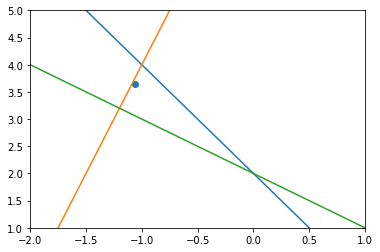
\includegraphics[width=0.7\linewidth]{figures/overdet_system}
	\caption{The three lines represent our system of equation, the point 
		the solution found with the pseudo-inverse technique.}
	\label{fig:overdet_system}
\end{figure}

Maybe you would have expected the point being at the barycenter of the
triangle, well this is not the case because the equations are not 
scaled the same way.


%To me the important property of the pseudo-inverse arises in solving a
%simple linear system of equations. It has 0, 1, or infinitely many
%solutions. \(𝑥=[𝐴]^+𝑏\) is the closest solution when none exists in the
%sense above. It gives the single answer when 1 exists. And when many
%exists, it is the smallest solution in the sense that \(||𝑥||_2\) is
%smallest.

\section{Principal Components Analysis}
\label{principal-components-analysis}

Principal Component Analysis, or PCA, is a dimensionality-reduction method that is often used to reduce the complexity of large datasets, by transforming the original set of variables into a smaller one that still contains most of the initial information.

Reducing the number of variables of a dataset naturally comes at the expense of accuracy. Since smaller datasets are easier to explore and visualize and make analyzing data simpler and faster without extraneous variables to process, hence the trick is to trade less accuracy for more simplicity

Let's see how this kind of technique can be implemented starting from 
a multidimensional initial dataset 
\begin{equation}
X=\begin{bmatrix}
x^{(1)}_1 &x^{(2)}_1&\cdots &x^{(m)}_1 \\
x^{(1)}_2 &x^{(2)}_2&\cdots &x^{(m)}_2 \\
\vdots &\vdots &\vdots &\vdots \\
x^{(1)}_n &x^{(2)}_n&\cdots &x^{(m)}_n 
\end{bmatrix}
\end{equation}

To allow an easier representation in the examples of this Section we will use the following two-dimensional dataset.

\begin{tcolorbox}[breakable, size=fbox, boxrule=1pt, pad at break*=1mm,colback=cellbackground, colframe=cellborder]
\begin{Verbatim}[commandchars=\\\{\}]
\PY{k+kn}{import} \PY{n+nn}{numpy} \PY{k}{as} \PY{n+nn}{np}
\PY{k+kn}{from} \PY{n+nn}{matplotlib} \PY{k}{import} \PY{n}{pyplot} \PY{k}{as} \PY{n}{plt}
	
\PY{n}{np}\PY{o}{.}\PY{n}{random}\PY{o}{.}\PY{n}{seed}\PY{p}{(}\PY{l+m+mi}{123}\PY{p}{)}
\PY{n}{x} \PY{o}{=} \PY{l+m+mi}{5}\PY{o}{*}\PY{n}{np}\PY{o}{.}\PY{n}{random}\PY{o}{.}\PY{n}{rand}\PY{p}{(}\PY{l+m+mi}{100}\PY{p}{)}
\PY{n}{y} \PY{o}{=} \PY{l+m+mi}{2}\PY{o}{*}\PY{n}{x} \PY{o}{+} \PY{l+m+mi}{1} \PY{o}{+} \PY{n}{np}\PY{o}{.}\PY{n}{random}\PY{o}{.}\PY{n}{randn}\PY{p}{(}\PY{l+m+mi}{100}\PY{p}{)}
	
\PY{n}{x} \PY{o}{=} \PY{n}{x}\PY{o}{.}\PY{n}{reshape}\PY{p}{(}\PY{l+m+mi}{100}\PY{p}{,} \PY{l+m+mi}{1}\PY{p}{)}
\PY{n}{y} \PY{o}{=} \PY{n}{y}\PY{o}{.}\PY{n}{reshape}\PY{p}{(}\PY{l+m+mi}{100}\PY{p}{,} \PY{l+m+mi}{1}\PY{p}{)}
	
\PY{n}{X} \PY{o}{=} \PY{n}{np}\PY{o}{.}\PY{n}{hstack}\PY{p}{(}\PY{p}{[}\PY{n}{x}\PY{p}{,} \PY{n}{y}\PY{p}{]}\PY{p}{)}
\end{Verbatim}
\end{tcolorbox}

Left plot of Fig.~\ref{fig:pca_dataset} shows the dataset.

\subsection{Standardization}
The first step to implement PCA is to standardize the range of the variables so that each one of them contributes equally.

More specifically, the reason why it is critical to perform \emph{standardization} prior to PCA, is that the latter is sensitive to the variances of the initial variables. That is, if there are large differences between the ranges of the variables, those with larger ranges will dominate over those with small ranges (e.g. a variable that goes from 0 and 100 will dominate over another one that ranges between 0 and 1), which will lead to biased results. 

Mathematically, this can be done by subtracting the mean and dividing by the standard deviation for each value of each variable

\begin{equation}
z = \cfrac{x - \textrm{mean}}{\textrm{std dev.}}
\end{equation}

Once the standardization is done, all the variables will be transformed to the same scale.

\begin{tcolorbox}[breakable, size=fbox, boxrule=1pt, pad at break*=1mm,colback=cellbackground, colframe=cellborder]
\begin{Verbatim}[commandchars=\\\{\}]
\PY{k}{def} \PY{n+nf}{centerData}\PY{p}{(}\PY{n}{X}\PY{p}{)}\PY{p}{:}
    \PY{n}{X} \PY{o}{=} \PY{n}{X}\PY{o}{.}\PY{n}{copy}\PY{p}{(}\PY{p}{)}
    \PY{n}{X} \PY{o}{=} \PY{p}{(}\PY{n}{X} \PY{o}{\PYZhy{}} \PY{n}{np}\PY{o}{.}\PY{n}{mean}\PY{p}{(}\PY{n}{X}\PY{p}{,} \PY{n}{axis} \PY{o}{=} \PY{l+m+mi}{0}\PY{p}{)}\PY{p}{)}\PY{o}{/}\PY{n}{np}\PY{o}{.}\PY{n}{std}\PY{p}{(}\PY{n}{X}\PY{p}{,} \PY{n}{axis}\PY{o}{=}\PY{l+m+mi}{0}\PY{p}{)}
    \PY{k}{return} \PY{n}{X}

\PY{n}{X\PYZus{}centered} \PY{o}{=} \PY{n}{centerData}\PY{p}{(}\PY{n}{X}\PY{p}{)}
\end{Verbatim}
\end{tcolorbox}

Right plot of Fig.~\ref{fig:pca_dataset} shows the standardized dataset
used in the following.

\begin{figure}[htb]
	\centering
	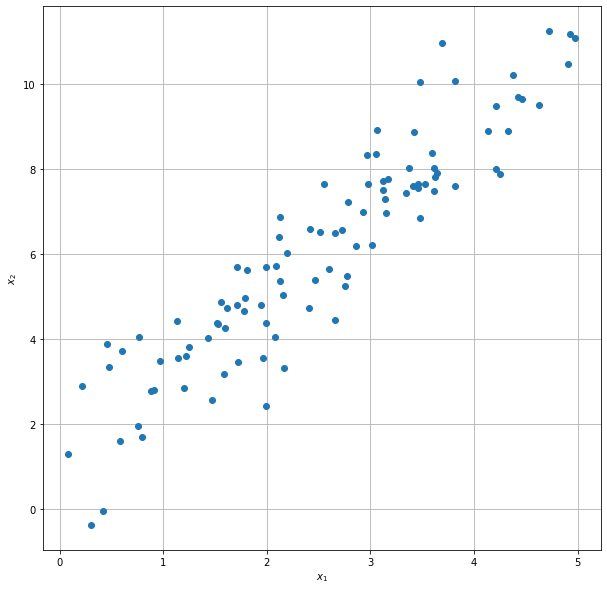
\includegraphics[width=0.45\linewidth]{figures/pca_dataset}
	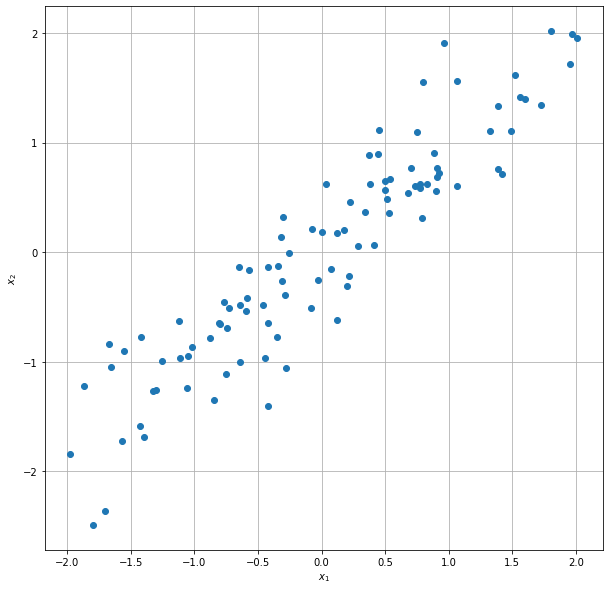
\includegraphics[width=0.45\linewidth]{figures/pca_dataset_centered}
	\caption{The dataset used in the PCA example (left), and
		the same dateset centered in the origin (right).}
	\label{fig:pca_dataset}
\end{figure}

\subsection{Covariance Matrix Computation}
The covariance matrix of our dataset helps us to understand if there 
is any relationship between the variables (i.e. sometimes, they are 
so correlated that they contain redundant information). So, in order to identify these correlations, we compute the covariance matrix.

The covariance matrix is a $n\times n$ (where $n$ is the number of dimensions) that has as entries the covariances associated with all possible pairs of the initial variables. Since the covariance of a variable with itself is its variance ($\textrm{cov}(a, a)= \textrm{var}(a)$), in the main diagonal (Top left to bottom right) we actually have the variances of each initial variable. And since the covariance is commutative ($\textrm{cov}(a, b) = \textrm{cov}(b, a)$), the entries of the covariance matrix are symmetric with respect to diagonal.

Once we have centered our data around 0, $[X^T][X]$ is the covariance matrix.

\begin{equation}
[\Sigma]=[X^T][X] =
\begin{bmatrix}
\textrm{var}(x_1) & \textrm{cov}(x_2, x_1) & \cdots & \textrm{cov}(x_n, x_1) \\
\textrm{cov}(x_1, x_2) & \textrm{var}(x_2) & \cdots & \textrm{cov}(x_n, x_2) \\
\vdots & \vdots & \vdots & \vdots \\
\textrm{cov}(x_1, x_n) & \textrm{cov}(x_2, x_n) & \cdots & \textrm{var}(x_n)
\end{bmatrix}
\end{equation}

\subsection{Principal Components}

Principal components are new variables that are constructed as linear combinations or mixtures of the initial variables. These combinations are done in such a way that the new variables (i.e. principal components) are uncorrelated and most of the information within the initial variables is squeezed or compressed into the first components. 

So, the idea is that a $n$-dimensional dataset gives you $n$ principal components, but PCA tries to put maximum possible information in the first component, then maximum remaining information in the second and so on.

Organizing information in principal components this way, will allow you to reduce dimensionality without losing much information, and this by discarding the components with low information and considering the remaining components as your new variables.
%An important thing to realize here is that, the principal components are less interpretable and don’t have any real meaning since they are constructed as linear combinations of the initial variables.

Geometrically speaking, principal components represent the directions of the data that explain a maximal amount of variance, that is to say, the lines that capture most information of the data. The relationship between variance and information here, is that, the larger the variance carried by a line, the larger the dispersion of the data points along it, and the larger the dispersion along a line, the more the information it has.

It is possible to demonstrate that the eigenvectors of the covariance matrix are actually the directions of the axis where there is the most variance (i.e. most information) and that we call \emph{principal components}. Eigenvalues are simply the coefficients, attached to eigenvectors, which give the amount of variance carried in each principal component.

As we have seen in Sec.~\href{find-eigenvalues-and-eigenvectors-in-python} the eigenvectors and eigenvalues of our dataset covariance are obtained as follows

\begin{tcolorbox}[breakable, size=fbox, boxrule=1pt, pad at break*=1mm,colback=cellbackground, colframe=cellborder]
\begin{Verbatim}[commandchars=\\\{\}]
\PY{n}{eigVals}\PY{p}{,} \PY{n}{eigVecs} \PY{o}{=} \PY{n}{np}\PY{o}{.}\PY{n}{linalg}\PY{o}{.}\PY{n}{eig}\PY{p}{(}\PY{n}{X\PYZus{}centered}\PY{o}{.}\PY{n}{T}\PY{o}{.}\PY{n}{dot}\PY{p}{(}\PY{n}{X\PYZus{}centered}\PY{p}{)}\PY{p}{)}
\PY{n+nb}{print} \PY{p}{(}\PY{n}{eigVecs}\PY{p}{)}
	
[[-0.70710678 -0.70710678]
 [ 0.70710678 -0.70710678]]

\PY{n+nb}{print} \PY{p}{(}\PY{n}{eigVals}\PY{p}{)}

[  7.46600865 192.53399135]
\end{Verbatim}
\end{tcolorbox}

If we rank the eigenvalues in descending order, we get $\lambda_2\gt\lambda_1$, which means that the eigenvector that corresponds to the first principal component (PC1) is  $v_2$ (i.e. the second column of the previous matrix).

After having the principal components, to compute the percentage of variance (information) accounted for by each component, we divide the eigenvalue of each component by the sum of eigenvalues. 

\begin{tcolorbox}[breakable, size=fbox, boxrule=1pt, pad at break*=1mm,colback=cellbackground, colframe=cellborder]
\begin{Verbatim}[commandchars=\\\{\}]
\PY{k}{for} \PY{n}{l} \PY{o+ow}{in} \PY{n}{eigVals}\PY{p}{:}
    \PY{n+nb}{print} \PY{p}{(}\PY{l+s+s2}{\PYZdq{}}\PY{l+s+si}{\PYZob{}:.1f\PYZcb{}}\PY{l+s+s2}{\PYZdq{}}\PY{o}{.}\PY{n}{format}\PY{p}{(}\PY{n}{l}\PY{o}{/}\PY{n}{np}\PY{o}{.}\PY{n}{sum}\PY{p}{(}\PY{n}{eigVals}\PY{p}{)}\PY{o}{*}\PY{l+m+mi}{100}\PY{p}{)}\PY{p}{)}
		
3.7
96.3
\end{Verbatim}
\end{tcolorbox}

If we apply this on the example above, we find that PC2 and PC1 carry respectively 96\% and 4\% of the variance of the data.

\subsection{Feature Vector}
Given the list of eigenvectors and eigenvalues we need to choose
whether to keep all these components or discard those of lesser significance (i.e. of low eigenvalues), and form with the remaining ones a matrix called \emph{feature vector}.

So, the feature vector is simply a matrix that has as columns the eigenvectors of the components that we decide to keep. This makes it the first step towards dimensionality reduction, because if we choose to keep only $p$ eigenvectors (components) out of $n$, the final dataset 
will have only $p$ dimensions.

Continuing with the example from the previous step, we can either form a feature vector with both of the eigenvectors $v1$ and $v2$, 
or discard the eigenvector $v_2$, which is the one of lesser significance, and form a feature vector with $v_1$ only.

Discarding the eigenvector $v_1$ will reduce dimensionality by 1, and will consequently cause a loss of information in the final data set. But given that $v_1$ was carrying only 4\% of the information, the loss will be therefore not important and we will still have 96\% of the information that is carried by $v_2$.

Figure~\ref{fig:pca_result} shows the two principal components.

\begin{figure}[htb]
	\centering
	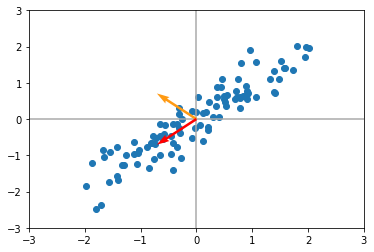
\includegraphics[width=0.7\linewidth]{figures/pca_result}
	\caption{The directions corresponding to the first two principal 
		components of our example dataset.}
	\label{fig:pca_result}
\end{figure}

\subsection{Recast Data Along Principal Components}
At this point we can use the feature vector to reorient data from the original axis to the ones represented by the principal components. 
This can be done by multiplying the transpose of the original dataset by the transpose of the feature vector

\begin{equation}
[Y] = [X^T][F^T]
\end{equation}

\begin{tcolorbox}[breakable, size=fbox, boxrule=1pt, pad at break*=1mm,colback=cellbackground, colframe=cellborder]
\begin{Verbatim}[commandchars=\\\{\}]
\PY{n}{Y} \PY{o}{=} \PY{n}{eigVecs}\PY{o}{.}\PY{n}{T}\PY{o}{.}\PY{n}{dot}\PY{p}{(}\PY{n}{X\PYZus{}centered}\PY{o}{.}\PY{n}{T}\PY{p}{)}
\end{Verbatim}
\end{tcolorbox}

The rotation transformed our dataset that have now the more
variance on one of the basis axis (i.e. the Cartesian axis). 
You could keep only this dimension
and have a fairly good representation of the data.
Figure~\ref{fig:pca_rotated} shows the effect of such a rotation to our
sample.

\begin{figure}[htb]
	\centering
	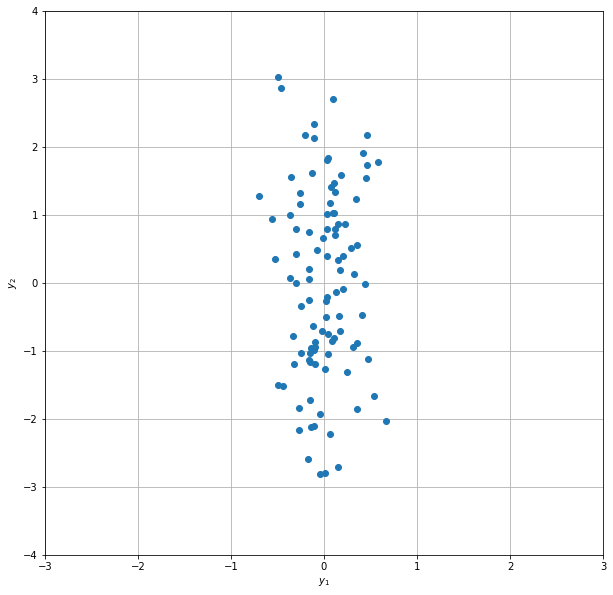
\includegraphics[width=0.5\linewidth]{figures/pca_rotated}
	\caption{The dataset rotated so that the usual Cartesian coordinates
		correspond to the first two principal components.}
	\label{fig:pca_rotated}
\end{figure}

\begin{thebibliography}{9}
%  %\bibitem{survey2019} StackOverflow \emph{The TEXbook}, Addison-Wesley, Reading,Massachusetts, second edition, 1984,

%[Steven M. Holland, Univ. of Georgia]: Principal Components Analysis
%[skymind.ai]: Eigenvectors, Eigenvalues, PCA, Covariance and Entropy
%[Lindsay I. Smith] : A tutorial on Principal Component Analysis
%Intuition Sean Owen - Pseudoinverse intuition Numpy Numpy - linalg.pinv

%Systems of equations Using the Moore-Penrose Pseudoinverse to Solve
%Linear Equations
%Overdetermined systems
%https://arxiv.org/pdf/1606.03899.pdf

%References PCA A lot of intuitive explanations on PCA
%Linear algebra - ncsu
%PCA - Ben-Gurion University
%SE - PCA objective function
%SE - Why do the leading eigenvectors of A maximize\ldots{}
\end{thebibliography}






